\documentclass[12pt]{article}
 
\usepackage[margin=1in]{}
\usepackage{amsmath,amsthm,amssymb,graphicx,geometry,mathtools,tikz,hyperref,outlines}

\usetikzlibrary{positioning}

\renewcommand{\d}[1]{\ensuremath{\operatorname{d}\!{#1}}}
\newcommand{\n}{\mathbb{N}}
\newcommand{\z}{\mathbb{Z}}
\newcommand{\q}{\mathbb{Q}}
\newcommand{\cx}{\mathbb{C}}
\newcommand{\real}{\mathbb{R}}
\newcommand{\field}{\mathbb{F}}
\newcommand{\ita}[1]{\textit{#1}}
\newcommand{\com}[2]{#1\backslash#2}
\newcommand{\oneton}{\{1,2,3,...,n\}}
\newcommand\idea[1]{\begin{gather*}#1\end{gather*}}
\newcommand\ef{\ita{f} }
\newcommand\eff{\ita{f}}
\newcommand\proofs[1]{\begin{proof}#1\end{proof}}
\newcommand\inv[1]{#1^{-1}}
\newcommand\setb[1]{\{#1\}}
\newcommand\en{\ita{n }}
\newcommand{\vbrack}[1]{\langle #1\rangle}
\newcommand\Inn{\mathrel{\ooalign{$\subset$\cr\hfil\scalebox{0.8}[1]{$=$}\hfil\cr}}}


\def\Plus{\texttt{+}}
\def\Minus{\texttt{-}}


\newenvironment{theorem}[2][Theorem]{\begin{trivlist}
\item[\hskip \labelsep {\bfseries #1}\hskip \labelsep {\bfseries #2.}]}{\end{trivlist}}
\newenvironment{lemma}[2][Lemma]{\begin{trivlist}
\item[\hskip \labelsep {\bfseries #1}\hskip \labelsep {\bfseries #2.}]}{\end{trivlist}}
\newenvironment{exercise}[2][Exercise]{\begin{trivlist}
\item[\hskip \labelsep {\bfseries #1}\hskip \labelsep {\bfseries #2.}]}{\end{trivlist}}
\newenvironment{reflection}[2][Reflection]{\begin{trivlist}
\item[\hskip \labelsep {\bfseries #1}\hskip \labelsep {\bfseries #2.}]}{\end{trivlist}}
\newenvironment{proposition}[2][Proposition]{\begin{trivlist}
\item[\hskip \labelsep {\bfseries #1}\hskip \labelsep {\bfseries #2.}]}{\end{trivlist}}
\newenvironment{corollary}[2][Corollary]{\begin{trivlist}
\item[\hskip \labelsep {\bfseries #1}\hskip \labelsep {\bfseries #2.}]}{\end{trivlist}}
 \hypersetup{
 colorlinks,
 linkcolor=blue
 }
\begin{document}

 
\title{Math 221 Notes}
\author{VOGEL, Max}
\date{UW-Madison, Summer 2020}

% https://tex.stackexchange.com/questions/186981/is-there-a-subsubsubsection-command
\setcounter{tocdepth}{4}
\setcounter{secnumdepth}{4}

\maketitle
\tableofcontents
\newpage

\section{Week 1}
\subsection{Day 1}
\subsubsection{Factoring:}
$$(a+b)(a^2-ab+b^2)=a^3+b^3 $$
$$(a-b)(a^2+ab+b^2)=a^3-b^3 $$


\subsubsection{Rules:}
\begin{minipage}{0.45\textwidth}
$$ a < b \rightarrow{} -a > -b $$
$$ -ax < b \rightarrow{} x > -\frac{b}{a} $$
$$ |x| = b \rightarrow{} x = b \vee x = -b $$
$$ |x| < b \rightarrow{} -b < x < b $$
$$ |x| = b \rightarrow{} x > b \vee x < -b $$
$$ a^m a^n = a^{m+n} $$
$$ \frac{a^m}{a^n} = a^{m-n}$$
$$ (ab)^m=a^m b^m$$
\hfill
\end{minipage}
\begin{minipage}{0.45\textwidth}
\begin{tabular}{|p{\textwidth}}
$$ \left(\frac{a}{b}\right)^n = \frac{a^n}{b^n}$$
$$ (a^m)^n = a^{mn}$$
$$ \sqrt{a} = a^{\frac{1}{2}}$$
$$ \sqrt[n]{a} = a^{\frac{1}{n}}$$
$$ \left(\sqrt[n]{a}\right)^m = \sqrt[n]{a^m} = a^{\frac{m}{n}}$$
$$ \sqrt{a}\sqrt{b} = \sqrt{ab}$$
$$ \sqrt[n]{a} \sqrt[n]{b} = \sqrt[n]{ab}$$\\
\end{tabular}
\end{minipage}

\subsubsection{Functions:}

\textbf{Definition: }
Assigns each element $x$ in a set $D$ exactly one element, called $f(x)$, in set $E$.\\
In terms of a graph, a curve can only be a function if no vertical lines intersect the curve more than once (vertical line test).
\begin{itemize}
    \item The set $D$ is called the domain -- possible $x$ values.
    \item The set $E$ is called the range -- possible $y$ values.
    \item If $f$ is a function with domain $D$, then it graph is the set of ordered pairs\\
    $ \{(x, f(x) | x) \text{ is a element of, } \in{}, D\}$
\end{itemize}
\paragraph{Finding domain:}
\begin{enumerate}
    \item $f(x) = \sqrt{x+2}$
    $\rightarrow{} x + 2 \geq{} 0$
    $\rightarrow{} x \geq{} -2 $
    $\rightarrow{} [-2, +\infty)$
    
    \item $f(x) = \frac{1}{x^2-x} $
    $\rightarrow{} x^2-x \neq{} 0 $
    $\rightarrow{} x(x-1) \neq{} 0 $
    $\rightarrow{} x \neq{} 0 \wedge x \neq 1 $
    $\rightarrow{} (-\infty, 0) \cup (0, 1) \cup (1, +\infty)$
\end{enumerate}

\paragraph{Picewise:}
\begin{itemize}
    \item Open circles, $\circ$, and circle brackets, ( ), are non-inclusive.
    \item Closed circles, $\bullet$, and square brackets, [ ], are inclusive.
    \item Formatted as: 
    \item[] $f(x)=\begin{cases} 
              y=5   : x < 0 \\
              y=x^2 : x\geq 0 
            \end{cases}$
\end{itemize}

\paragraph{Types}
\begin{itemize}
    \item[] \textbf{Even: }
    \item A function is even if $f(x) = f(-x)$
    \item The graph is symmetric with respect to the y-axis.
    \item Examples: $x^4 - 2, x^{20}+x^6, \cos(x), |x|$

\end{itemize}

\begin{itemize}
    \item[] \textbf{Odd: }
    \item A function is even if $f(x) = -f(x)$
    \item The graph has rotational symmetry about origin.
    \item Examples: $x^3, x^{7}+x, \sin(x), |x|x$
\end{itemize}

\noindent\hrulefill

\begin{itemize}
    \item[-] Even times odd function is always odd.
    \item[-] Even times even is always even.
    \item[-] Odd times odd is always even.
\end{itemize}

\paragraph{Increasing \& Decreasing:}
\begin{itemize}
\item \textbf{Increasing :} A  function $f$ is called increasing on an interval if $f(x_1) < f(x_2)$ whenever $x_1 < x_2$. In other words, the slope must always be positive.
\item \textbf{Decreasing :} A  function $f$ is called increasing on an interval if $f(x_1) > f(x_2)$ whenever $x_1 < x_2$. In other words, the slope must always be negative.
\end{itemize}


\subsubsection{Limits}

\textbf{Definition: } Supposing $f(x)$ is defined when $x$ is near the number $a$, we write $\lim_{x\to a} f(x) = L$ and say ``the limit of $f(x)$, as $x$ approaches $a$, equals $L$''.


\begin{itemize}
    \item $\lim_{x\to a} f(x) = L$ if and only if (iff, $\iff$) $\lim_{x\to a^-} f(x) = L \wedge \lim_{x\to a^+} f(x) = L$
    \item That is, the limit does not exist, $\nexists$, if $x$ approaches different values when from the left and right sides 
    \item Approaching from left (from $-\infty \to \infty$) is notated as $x \to a^-$
    \item Approaching from right (from $\infty \to -\infty$)) is notated as $x \to a^+$
    \item iff, $\iff$:
        $$A \iff B \rightarrow{}$$
        $$A \text{ is necessary and sufficient for B }\rightarrow{}$$
        $$B \text{ is necessary and sufficient for A } \rightarrow{}$$
        $$A \text{ is equivalent to } B$$
    \item A vertical asymptote exists if the limit from left side is $+\infty$ or $-\infty$, and the limit from the right side is the opposite.
\end{itemize}

\paragraph{Infinite Limits}
\begin{itemize}
    \item If function limit is $\pm \infty$ (if the denominator is 0 at $f(a)$), you can find whether its $\Plus{}$ or $\Minus{}$ by solving the limit for each term. If the term is positive, then it's $+ \infty$, and vice-versa, e.g.
    
    $$\lim_{x \to -2^+} \frac{x-1}{x^2(x+2)}$$
    $$\frac{\lim_{x \to -2^+} [x-1]}{ (\lim_{x \to -2^+} [x])^2 \cdot \lim_{x \to -2^+} [(x+2)]}$$
    $$\frac{\ominus}{\oplus \cdot \oplus}$$
    $$\ominus \rightarrow{} -\infty$$

\end{itemize}

\subsubsection{Lines}
\begin{itemize}
    \item Slope-Point form: $y-b = m(x+a)$ -- $(a,b)$ will be a point of the equation.
    \item Slope-Intercept form: $y = mx + b$ -- $(0,b)$ will be the $y$-intercept.
    \item Vertex form: $y = a(x-h)+k$ -- $(h,k)$ will be the vertex.
    \item Point-Point form: $y-y_1=\frac{y_2-y_1}{x_2-x_1}(x-x_1)$ -- $(x_1,y_1)$ and $(x_2,y_2)$ will be points of the equation.
    \item Intercept form:  $\frac{x}{a} + \frac{y}{b} = 1$  -- $(a, b)$ will be a point of the equation.
    
\end{itemize}

\subsection{Day 2}
\subsubsection{Limit Laws:}
Supposing $c$ is a constant and $\lim_{x \to a}f(x)$ and $\lim_{x \to a}g(x)$ exists, then\\
\begin{minipage}{0.5\textwidth}
    $$\lim_{x \to a} [f(x) \pm g(x)] = \lim_{x \to a} f(x) \pm \lim_{x \to a} g(x)$$
    $$\lim_{x \to a} [cf(x)] = c \cdot \lim_{x \to a} f(x)$$
    $$\lim_{x \to a} [f(x)g(x)] = \lim_{x \to a} f(x) \lim_{x \to a} g(x)$$
    $$\lim_{x \to a} \left [ \frac{f(x)}{g(x)} \right ] = \frac{\lim f(x)}{\lim g(x)} \text{ if } \lim_{x \to a} g(x) \neq{} 0$$
    $$\lim_{x \to a} [f(x)]^n = [\lim_{x \to a} f(x)]^n$$

\hfill
\end{minipage}
\begin{minipage}{0.45\textwidth}
\begin{tabular}{|p{\textwidth}}
$$\lim_{x \to a} c = c$$
$$\lim_{x \to a} x = a$$
$$\lim_{x \to a} x^n = a^n \text{ where } n = \mathbb{Z}^+$$ 
$$\lim_{x \to a} \sqrt[n]{x} = \sqrt[n]{a} \text{ where } n = \mathbb{Z}^+$$ 
$$\lim_{x \to a} \sqrt[n]{f(x)} = \sqrt[n]{f(a)} \text{ if } f(a) \geq 0 \text{ and } n_{even}$$
\end{tabular}
\end{minipage}

\noindent\textbf{Direct Substitution Property:} If $f$ is a polynomial or rational function, and $a$ is in the domain of $f$, then $\lim_{x \to a} f(x) = f(a)$\\
\textbf{Theorem 1.6.1:} If $f(x) = g(x)$ when $x \neq a$, then $\lim_{x\to a} f(x) = \lim_{x\to a} g(x)$ \\
\textbf{Theorem 1.5.1:} If $f(x) = L \iff \lim_{x\to a^-} f(x) = L = \lim_{x\to a^+} f(x)$\\
\textbf{Theorem 1.6.2:} If $f(x) \leq g(x)$ when $x$ is near $a$ and the limits of $f$ and $g$ both exist as $x$ approaches $a$, then $\lim_{x\to a} f(x) \leq \lim_{x\to a} g(x)$\\
\textbf{Squeeze Theorem:} If $f(x) \leq g(x) \leq h(x)$ when $x$ is near $a$ and 
 $\lim_{x\to a} f(x) =  \lim_{x\to a} h(x) = L$, then $\lim_{x\to a} g(x) = L$


\subsubsection{Piecewise / $(\epsilon, \delta)$ definition  of limit}
If for every small number $\epsilon >  0$ there is a number $\delta > 0$ such that if $0 < |x-c| < \delta$ then $|f(x) - L| < \epsilon$.

$$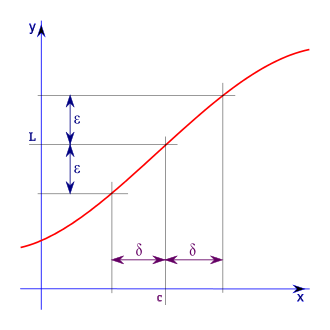
\includegraphics[width=0.5\textwidth]{media/limit01.png}$$

\noindent Solving for $\delta$, rewrite the term defining $\epsilon$ to be equal to the term defining $\delta$. E.g., solving for $\delta$ if $|x-2|<\delta$, then $|4x-8|<\epsilon$, where $\epsilon = 0.1$:

$$|4x-8|=4|x-2|<0.1$$
$$|x-2| < \frac{0.1}{4}\text{, therefore } \delta=\frac{0.1}{4}$$

\noindent For non-linear equations, find the lesser and greater $\delta$, and choose the one that results in the smaller $\epsilon$.

\subsection{Day 3}
\subsubsection{Continuous Function:}
\textbf{Definition:} A function $f$ is continuous at  a number if $\lim_{x\to a} f(x) = f(a)$. Graphically, a function is continuous if you can draw it without having your pen leave paper. More formally, $f(x)$ is continuous at $x=a \iff:$ 

\begin{enumerate}
    \item $f(a)$ is defined ($a \in{} D: $ $a$ is in the domain of $f$).
    \item $\lim_{x\to a} f(x)$ exists, and equals $f(x) = f(a)$.
\end{enumerate}

If one of the aforementioned statements is incorrect, then $f(x)$ is discontinuous at $x=a$

\textbf{Theorem 1:} A function is continuous on an interval if it's continuous at every number in the interval. That is, if $f$ and $g$ are continuous at $x=a$, then the following are also continuous at $a$:\\
$$f+g, f-g, cf, fg, \frac{f}{g} \text{ for } g(a) \neq{} 0$$


\textbf{Theorem 2:} The following types of functions are continuous at every number in there domain: Polynomials, Rational functions, Root functions, \& Trig functions.\\


\textbf{Theorem 3: Intermediate Value Theorem (IVM):} Suppose that $f$ is continuous on the close interval $[a,b]$ and let $N$ be any number between $f(a)$ and $f(b)$, where $f(a) \neq{} f(b)$. Then there exists at least on number $c$ in $(a,b)$ such that $f(c)=N$. 

$$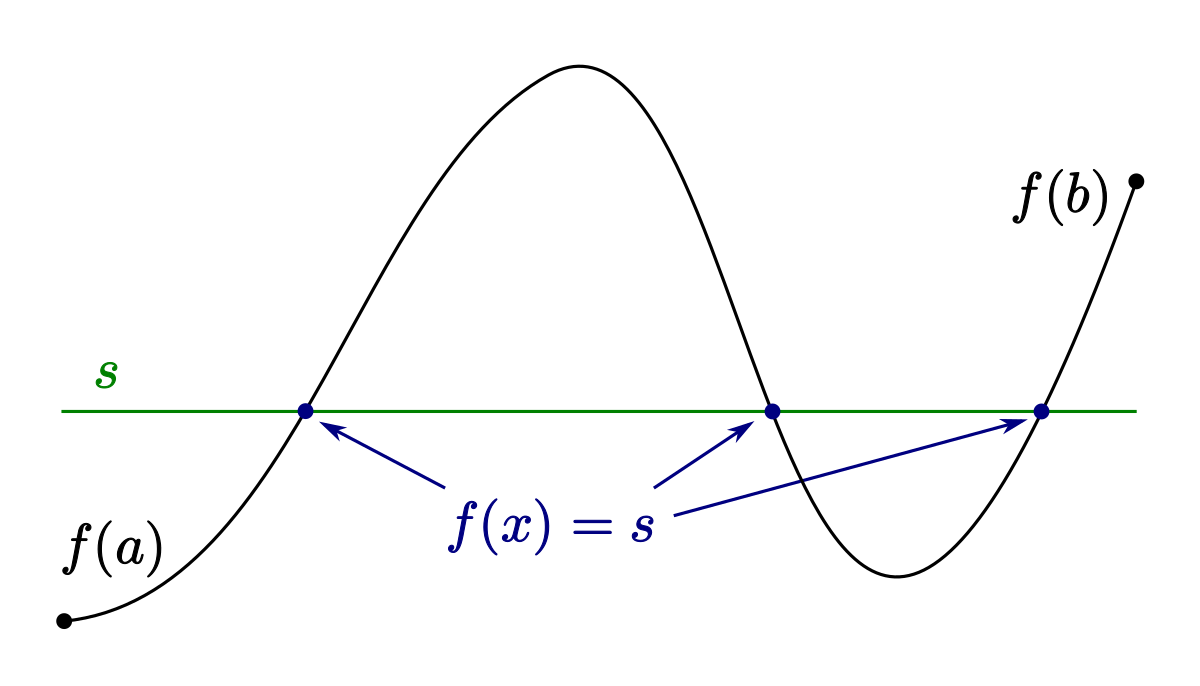
\includegraphics[width=0.5\textwidth]{media/ivm.png}$$

\subsection{Day 4}
\subsubsection{Lines:}
\paragraph{Secant Line:} A line that locally intersects two points on a curve.

$$\frac{\text{Rise}}{\text{Run}} = \frac{\Delta y}{\Delta x} = \frac{y_1 - y_0}{x_1 - x_0} =  \frac{f(a+h)-f(a)}{(a+h)-a}=\frac{f(a+h)-f(a)}{h}$$

$$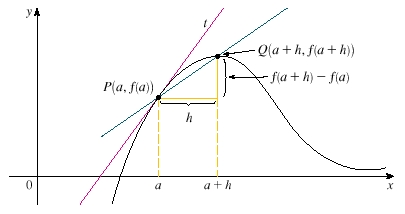
\includegraphics[width=0.65\textwidth]{media/secanteq.jpg}$$

\paragraph{Tangent Line:} The line through a pair of infinitely close points on the curve so that the line is ``just touching''. Slope equation (also known as ``Difference Quotient''):

$$\lim_{h \to 0} \left [ \frac{f(a+h)-f(a)}{h} \right ]$$

\subsubsection{Derivatives:} The derivative of a function $f$ at a number $a$, denoted by $f'(a)$, is 

$$f'(a) = \lim_{h \to 0} \left [ \frac{f(a+h)-f(a)}{h} \right ]$$
and the equation of the tangent line to the curve $y=f(x)$ at the point $(a,f(a))$ can be written in point-slope form as

$$y-f(a)=f'(a)(x-a)$$

\section{Week 2}
\subsection{Day 5}
\subsubsection{Derivatives (cont.):}
\begin{itemize}
    \item Other notation is $\frac{d y}{d x} |_{x=a}$ (Leibniz Notation),  $\frac{d f}{d x}$, $\frac{d}{d x}$ $f(x)$, $f(x)$, $D f(x)$, \& $D_{x} f(x)$
    \item Function $f(x)$ is differentiable at $x=a$ if $f'(a)$ exists (same as Theorem 1.5.1).
    \item Therefore, Not Continuous $\implies$ Not Differentiable.
    \item If $f'(a)$ exists, then $\lim_{x \to a} f(x) = f(a)$
    \item The derivative is a function, not a constant.
    \item Because $f'$ is also a function, $f'$ may have a derivative of its own, denoted by $(f')' = f''$ and called the \textbf{second derivative} of $f$. This can also be written as $\frac{d}{d x} \left ( \frac{d y}{d x} \right ) = \frac{d^2 y}{dx^2}$
\end{itemize}


\subsection{Day 6}
\subsubsection{Derivatives Rules:}

\begin{minipage}{0.5\textwidth}

\begin{itemize}
    \item Constant: $\frac{d}{d x}(c) = 0$
    \item Linear: $\frac{d}{d x}(x) = 1$
\end{itemize}

\end{minipage}
\begin{minipage}{0.45\textwidth}
\begin{tabular}{|p{\textwidth}}
\begin{itemize}
    \item Linear + Constant: $\frac{d}{d x}(ax) = a$
    \item Power Rule: $\frac{d}{d x}(x^n) = n x^{n-1}$
\end{itemize}
\end{tabular}
\end{minipage}

\begin{itemize}
    \item Constant Multiple: $\frac{d}{d x}[c \cdot f(x)] = c \cdot \frac{d}{d x}(f(x))$
    \item Sum/Difference: $\frac{d}{d x}[f(x) \pm g(x)] = f'\pm g'$
    \item Product Rule: $\frac{d}{d x}[f(x)\cdot g(x)] = f'\cdot g + f \cdot g'$
    \item Quotient Rule: $\frac{d}{d x}\left[ \frac{f(x)}{g(x)} \right] = \frac{g\cdot f'- f\cdot g'}{g^2} = \frac{\text{lo} \cdot \text{d hi - hi} \cdot \text{d lo}}{\text{lo}\cdot\text{lo}}$
\end{itemize}

\subsubsection{Lines:}
\textbf{Theorem:} If the graph of $y=m_1x+b_1$ is perpendicular to the graph of $y=m_2x+b_2$, then $m_1m_2 = -1$. 
\\
\textbf{Normal Line:} The normal line to a curve at point $M$ is the line through $M$ that is perpendicular to the tangent line at $M$.

$$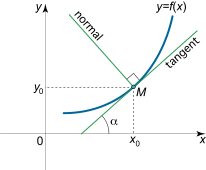
\includegraphics[width=0.5\textwidth]{media/normal-tangent.png}$$


\subsection{Day 7}
\subsubsection{Trig Review:}
$$\csc = \frac{1}{\sin}, \ \sec = \frac{1}{\cos}, \ \cot = \frac{1}{\tan} = \frac{\cos}{\sin}$$
\subsubsection{Trig Identities:}
$$\sin^2 + \cos^2 = 1$$
$$\text{Dividing by }\sin^2: 1 + \frac{\cos^2}{\sin^2} = \frac{1}{\sin^2} \rightarrow{} 1 + \cot^2 = \csc^2$$
$$\text{Dividing by }\cos^2: \frac{\sin^2}{\cos^2} + 1 = \frac{1}{\cos^2} \rightarrow{} \tan^2 + 1 = \sec^2$$
\subsubsection{Derivative of Trig Functions:}
\begin{minipage}{0.5\textwidth}
    
    $$(\sin)' = \cos$$
    $$(\cos)' = -\sin$$
    $$(\tan)' = \sec^2 $$
\hfil
\end{minipage}
\begin{minipage}{0.45\textwidth}
\begin{tabular}{|p{\textwidth}}

    $$(\csc)' = -\cot \cdot \csc$$
    $$(\sec)' = \sec \cdot \tan$$
    $$(\cot)' = -\csc^2 $$

\end{tabular}
\end{minipage}

\subsubsection{Limit of Trig Functions:}

$$\lim_{\theta \to 0}{\frac{\sin \theta}{\theta}} = 1$$

\section{Week 3}
\subsection{Day 9}
\subsubsection{Composite Function: } A new function can be  composed to two old functions, such as $f \circ g$. Formally, given two functions $f$ and $g$, the composite function $f \circ g$ and $g \circ f$ (also called the composition of $f$ and $g$) is defined by $(f \circ g)(x)  = f(g(x))$ and $(g \circ f)(x)  = g(f(x))$

\subsubsection{Decomposite Function: } Many functions can be decomposed into small functions, $h(x) = f(g(x))$

\subsubsection{Chain Rule} If the composite function $F(x) = f \cdot g$ is defined by $F(x) = f(g(x))$ is differentiable at $x$ and $F'$ is given by the product 

$$F'(x) = f'(g(x)) \cdot g'(x) \text{ or } OUT'(in) \cdot IN'$$

\noindent\text{The power rule can be combined with the chain rule as}

$$\frac{d}{dx}[g(x)]^n = n[g(x)]^{n-1} \cdot g'(x)$$


\subsection{Day 10}

\subsubsection{Explicit and Implicit:}
\textbf{Explicit: } A function given in terms of the independent variable, e.g. $y=\sqrt{x^3+1}$.\\
\textbf{Implicit: } A function given in terms of both dependent and independent variables, e.g. $x^3-y^2+1=0,\ y \geq 0$.\\
\textbf{Implicit Differentiation: } If the function is stuck in implicit form, then differentiate both sides of the equation with respect to $x$ and solve the resulting equation for $y'$.\\
\textbf{Note: }
$$\frac{d}{dx}(y^n) \neq{} ny^{n-1}  \ \ \ \ \ \ \frac{d}{dx}(y^n) = ny^{n-1} \cdot y'$$

\subsection{Day 11}
\subsubsection{Related Rates:}
A related rates problem is to compute the rate of change (derivative) of one quantity in terms of the rate of change of another quantity, which is more easily measured.
\\\\
\noindent How to approach a related rates problem:
\begin{enumerate}
    \item Read the problem, and draw a diagram if possible.
    \item Assign symbols to all variables that are a function of time.
    \item Find an equation that relates the two variables.
    \item Using the Chain Rule to differentiate both sides with respect to time.
    \item Substitute the given information into resulting equation and solve for the unknown
    rate.
\end{enumerate}

\subsection{Day 12}
\subsubsection{Maximum and Minimum Values:}
\textbf{Absolute or Global [Max/Min]: } The [max/min] $y$-value in the domain. \\
\textbf{Relative or Local [Max/Min]: } The [max/min] $y$-value in a given range around a $x$-value. Can only occur when the graph goes from [increasing to decreasing / vice-versa]\\
\textbf{Note: } The endpoint of a graph can never be a relative [max/min] because one side of the point is always undefined. 

\subsubsection{Increasing/Decreasing Functions:}
$$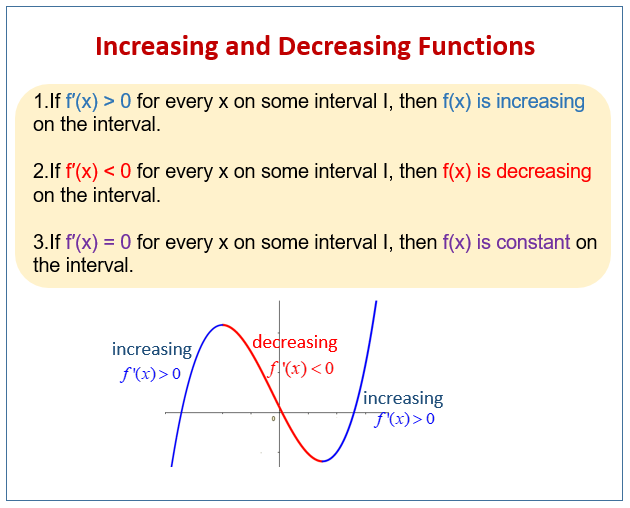
\includegraphics[scale=.75]{media/increasing-decreasing-functions.png}$$


\subsubsection{Concavity:}
$$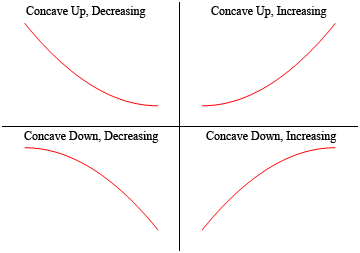
\includegraphics[scale=.75]{media/concavity.png}$$

\subsubsection{Extreme Value Theorem:} Suppose that $f(x)$ is continuous on the interval $[a,b]$ then there are two numbers, $a \leq c, d \leq d$ so that $f(c)$ is an absolute maximum for the function and $f(d)$ is an absolute minimum for the function.

\subsubsection{Fermat's Theorem:} If $f$ has a local max or min at $a$, and $f'(a)$ exists, then $f'(a) = 0$.

\subsubsection{Critical Number: } A critical number of a function $f$ is a number $c$ in the domain of $f$ such that either $f'(c) = 0$ or $f'(c) = $ DNE

\subsubsection{Absolute Extreme: } To find the absolute max and min values of a continuous function $f$ on a closed interval $[a,b]$: 

\begin{enumerate}
    \item Find the critical numbers of the function on $(a,b)$
    \item Find the values of $f$ at the critical numbers of $f$ in $(a,b)$
    \item Find the values of $f$ at the end points of the interval, in other words, find $f(a)$ and $f(b)$.
    \item The largest of the values from steps 2 and 3 is the absolute max, the smallest is the absolute min.
    
\end{enumerate}

\section{Week 3}
\subsection{Day 13}
\subsubsection{Rolle's Theorem} Let $f$ be a function that satisfies the following three hypotheses:
\begin{enumerate}
    \item $f$ is continuous on the closed interval $[a,b]$
    \item $f$ is differentiable on the open interval $(a,b)$
    \item $f(a) = f(b)$
\end{enumerate}
Then there is at least one number $c$ in $(a,b)$ such that $f'(c) = 0$

$$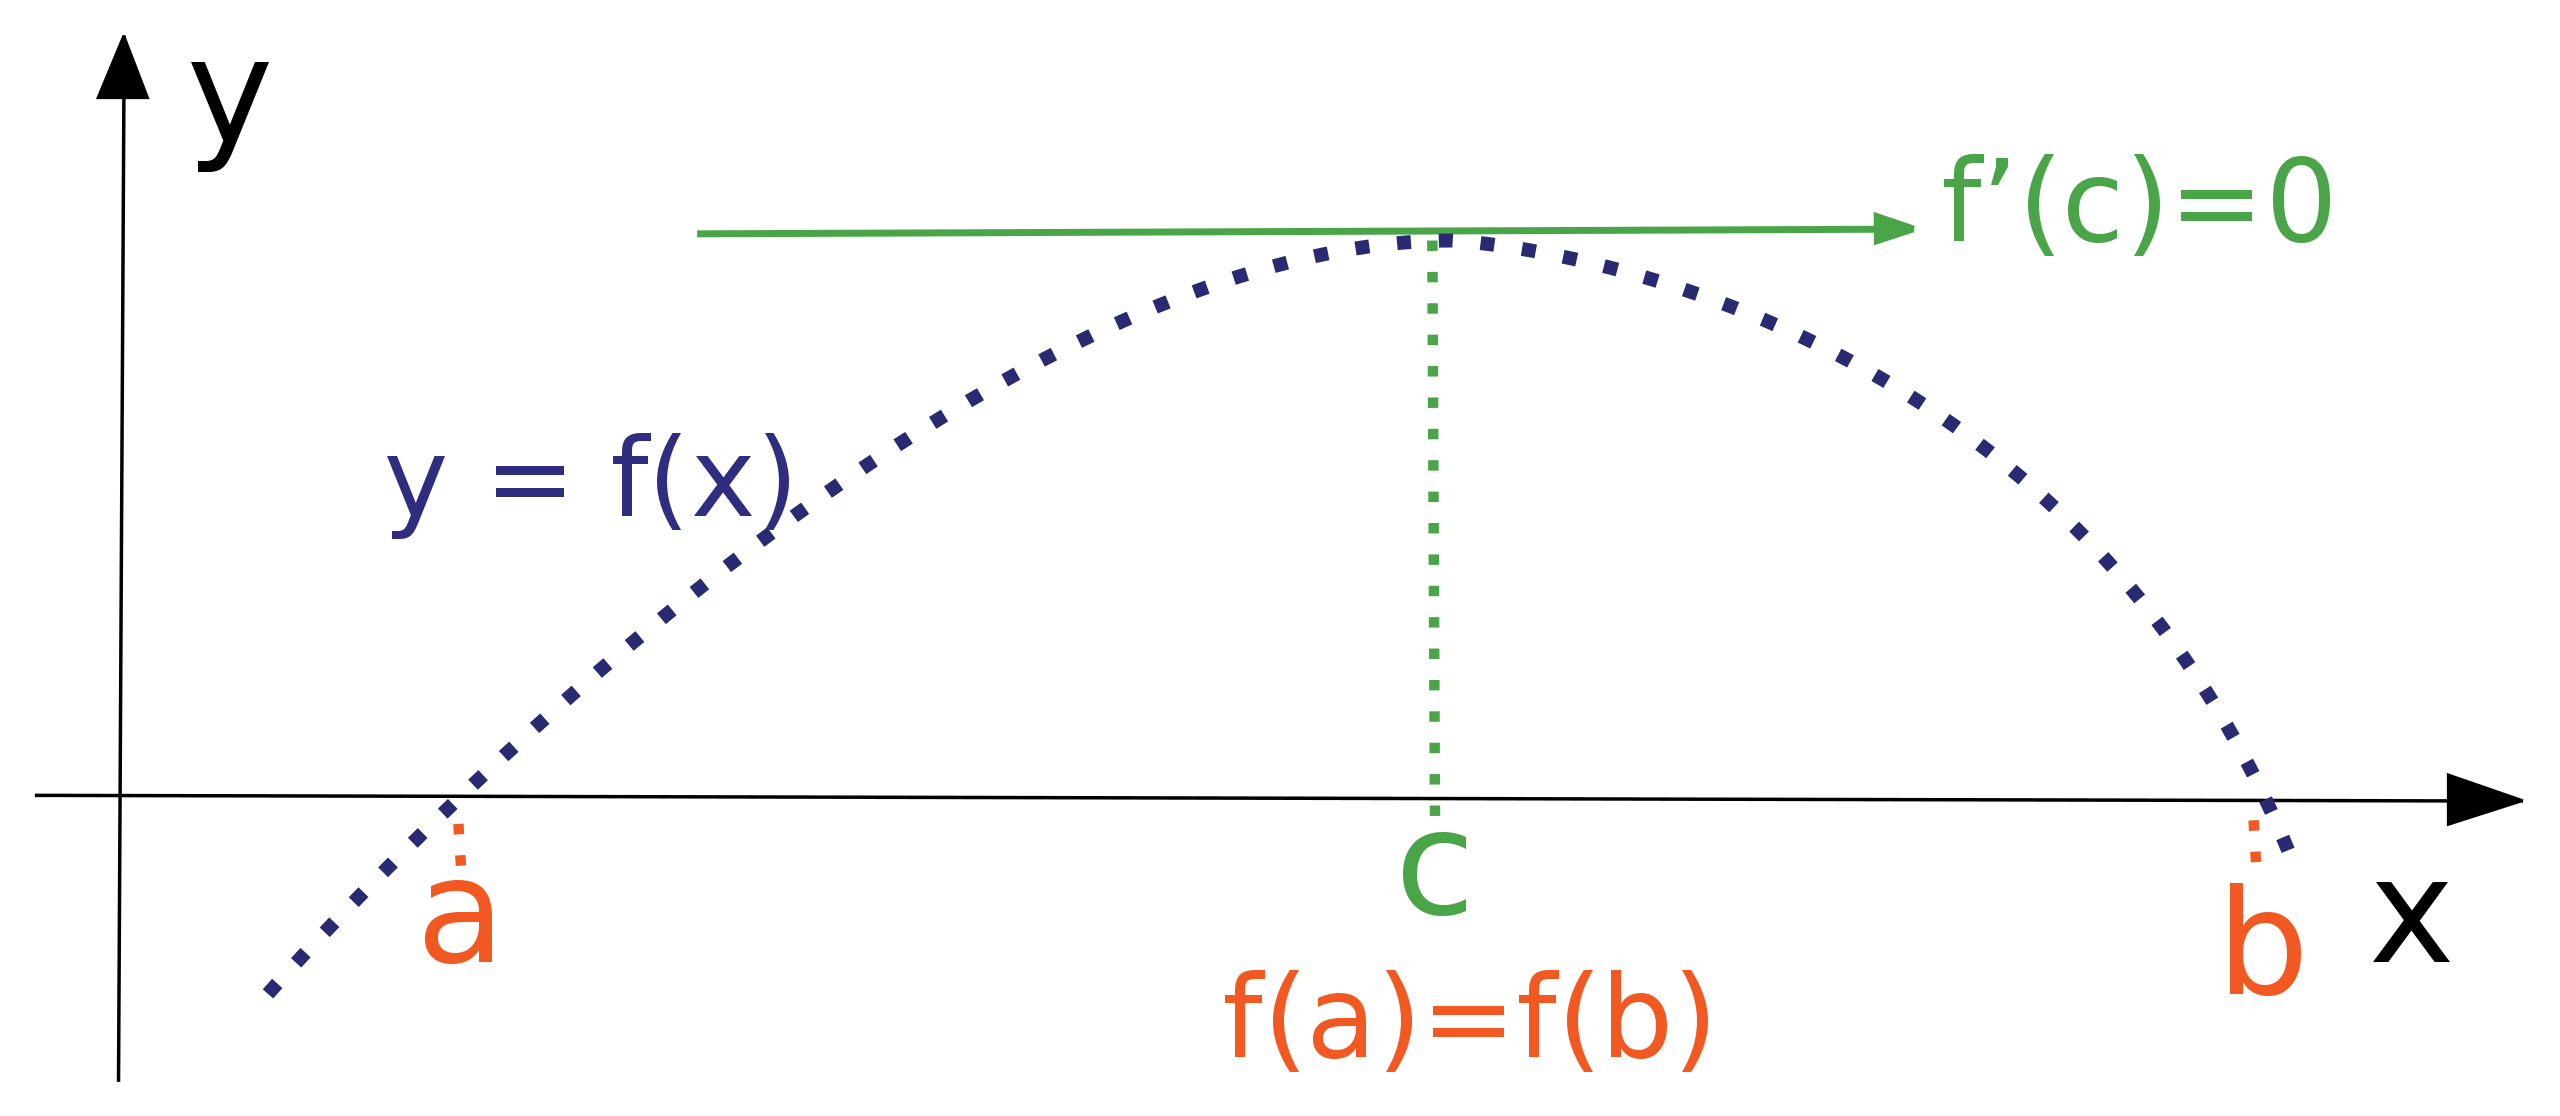
\includegraphics[width=0.7\textwidth]{media/rolles.png}$$

\paragraph{Proof}
\begin{itemize}
    \item Case 1: $f(x) = k, $ a constant. Then, $f'(x) = 0$ so the number $c$ can be taken to be any number in $(a,b)$.
    \item Case 2: $f(x) > f(a), $ concave down, for some $x$ in $(a,b)$. By the extreme value theorem, $f$ has a max value in $[a,b]$. Since $f(a)=f(b)$, it must attain it's max value at $c$; $c \in (a,b)$. Then, $f$ has a local max at $c$, $f$ is differentiable at $c$, therefore $f'(c)$ = 0 by Fermat's theorem. 
    \item Case 3: $f(x) < f(a), $ concave up, for some $x$ in $(a,b)$. By the extreme value theorem, $f$ has a min value in $[a,b]$. Since $f(a)=f(b)$, it must attain it's min value at $c$; $c \in (a,b)$. Then, $f$ has a local min at $c$, $f$ is differentiable at $c$, therefore $f'(c)$ = 0 by Fermat's theorem. 
\end{itemize}

\subsubsection{Mean Value Theorem} Let $f$ be a function that satisfies the following hypotheses: 

\begin{itemize}
    \item $f$ is continuous on the closed interval $[a,b]$
    \item $f$ is differentiable on the open interval $(a,b)$
\end{itemize}

Then there is at least one number $c$ in $(a,b)$ such that $$f'(c)=\frac{f(b)-f(a)}{b-a}$$
$$\text{Slope of tangent line at } c = \text{Slope of Secant Line} $$
$$f(b) - f(a) = f'(c)(b-a)$$

$$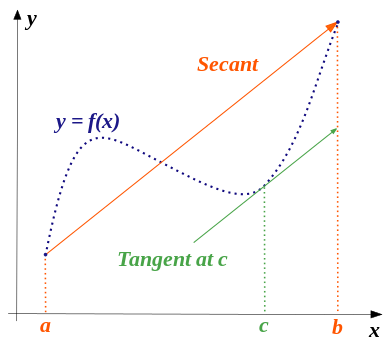
\includegraphics[width=0.7\textwidth]{media/mvt.png}$$

\subsection{Day 14}
\subsubsection{Determining Increasing/Decreasing: }
\begin{enumerate}
    \item Find the critical numbers
    \item Mark the critical numbers on a real line
    \item Pick a test number, $c$, in each interval:
    \item[$\cdot$] If $f'(c) > 0$, $f$ is increasing at that interval
    \item[$\cdot$] If $f'(c) < 0$, $f$ is decreasing at that interval
\end{enumerate}

\subsubsection{Local max and min: }
\begin{enumerate}
    \item Find the critical numbers
    \item Mark the critical numbers on a real line
    
    \item Pick a test number, $c$, in each interval:
    \item[$\cdot$] If $f'$ changes from $\oplus$ to $\ominus$, then $f$ has a local max at $f(c)$
    \item[$\cdot$] If $f'$ changes from $\ominus$ to $\oplus$, then $f$ has a local min at $f(c)$
    \item[$\cdot$] If $f'$ doesn't change sign, then $f$ has no local min or min at $f(c)$
\end{enumerate}

\subsubsection{Second Derivative Test} Suppose $f''$ is continuous near $c$. 
\begin{enumerate}
    \item If $f'(c) = 0$ and $f''(c) < 0$, then $f$ has a local max at $c$.
    \item If $f'(c) = 0$ and $f''(c) > 0$, then $f$ has a local min at $c$.
    \item If $f'(c) = 0$ and $f''(c) = 0$, then the second derivative test says nothing about the point $c$, a possible inflection point
\end{enumerate}
\subsubsection{Finding Concavity}
\begin{enumerate}
    \item $f(x)$ increasing implies $f'(x)>0$
    \item $f'(x)$ increasing implies $f''(x)>0$
    \item $f''(x)>0$ for all $x$ in $I$, then the graph of $f$ is concave upwards on $I$
    \item $f''(x)<0$ for all $x$ in $I$, then the graph of $f$ is concave downwards on $I$
\end{enumerate}

\paragraph{Inflection Point:} A point $p$ on a curve $f(x)$ is called an inflection point if $f$ is continuous there and the curve changes at $p$ from concave up to concave down or vice versa.

\paragraph{Theorem:} At a point of inflection, $(c, f(c))$, either $f''(c)=0$ or $f''(c)$ DNE.

\subsection{Day 15}
\subsubsection{Limit at $\infty{}$} Let $f$ be a function defined on some interval $(a, +\infty{})$. Then $\lim_{x \to \infty{}} f(x) = L$ means that the value of $f(x)$ can be made arbitrarily close to $L$ by making $x$ sufficiently large. In other words, for every $\epsilon > 0$, there is a number $N$ such that if $x<N$ then $|f(x)-L| < \epsilon$. "$N$": Large negative number.

\subsubsection{Horizontal Asymptote} The line $y=L$ is called a  horizontal asymptote of the curve $y=f(x)$ if either $\lim_{x \to +\infty{}} f(x) = L$ or $\lim_{x \to -\infty{}} f(x) = L$

\paragraph{Theorem} If $r>0$ is a rational number, then $\lim_{x \to \infty{}} \frac{1}{x^r} = 0$\\
If $r>0$ is a rational number such that $x^r$ is defined for all $x$, then $\lim_{x \to -\infty{}} \frac{1}{x^r} = 0$


\section{Week 5}

\subsection{Day 17} 
\subsubsection{Optimization} 
\begin{enumerate}
    \item Understand the problem. What is the unknown? What are the given quantities? What are the given conditions?
    \item Draw a diagram.  Show variables.
    \item Introduce notation. Assign $Q$ to the quantity that is to be maximized or minimized.
    \item Express $Q$ in terms of other variables.
    \item If $Q$ is expressed with more than one variable, use the given info to find a relationship among these variables.
    \item Find the absolute max or min value of the $Q$ (the function). 
\end{enumerate}


\subsection{Day 18}
\subsubsection{Area Under Curve: } The area $A$ of the region $S$ that lies under the graph of the continuous function $f$ is the limit of the sum of the areas of approximating rectangles:

$$A=\lim_{n\to \infty} R_n = \lim_{n\to \infty} (f(x_1)\Delta x) + f(x_2)\Delta x) + ... + f(x_n)\Delta x) = \lim_{n\to \infty} \sum_{i=1}^{n} f(x_i)\Delta x$$
$$A=\lim_{n\to \infty} r_n = \lim_{n\to \infty} (f(x_0)\Delta x) + f(x_1)\Delta x) + ... + f(x_{n-1})\Delta x)= \lim_{n\to \infty} \sum_{i=1}^{n} f(x_{i-1})\Delta x$$

\subsubsection{Absolute Extreme Values} Suppose that $c$ is a critical number of a continuous function $f$ defined on an interval. 
\begin{itemize}
    \item If $f'(x)>0$ for all $x<c$, and $f'(x)<0$ for all $x>c$, then $f(c)$ is the absolute max for values of $f$.
    \item If $f'(x)<0$ for all $x<c$, and $f'(x)>0$ for all $x>c$, then $f(c)$ is the absolute min for values of $f$.
\end{itemize}

\subsubsection{Anti-derivative}
A function $F$ is called an antiderivative of $f$ on an interval $I$ if $F'(x) = f(x)$ for all $x$ in $I$.

\noindent For example, $F(x)=x^3$ and $f(x) = 3x^2$:
\begin{itemize}
    \item $f(x)$ is derivative of function $F(x)$
    \item $F(x)$ is antiderivative of function $f(x)$
\end{itemize}

\paragraph{Theorem} If $F$ is an antiderivative of $f$ on an interval $I$, then the most general antiderivative of $f$ on $I$ is $F(x)+C$ where $C$ is an arbitrary constant.

\paragraph{Initial Condition Steps}
\begin{enumerate}
    \item Find the anti-derivative of $f(x)$
    \item Plug in the initial  condition to evaluate constant $C$
    \item Find the solution
\end{enumerate}

\subsubsection{Differential Equations} An equation that involves the derivatives of a function is called a differential equation.\\
The solution of a differential equation is a function that satisfies the equation. 

\subsection{Day 19}

\subsubsection{Definite Integral} 

If $f$ is continuous on $[a,b]$, or if $f$ has only a finite number of jump discontinuities, then $f$ is integrable on $[a,b]$; that is, the definite integral exists.
$$\int_a^b f(x) dx=\lim_{n\to \infty} \sum_{i=1}^{n} f(x_i^*)\Delta x$$


\paragraph{Properties}

$$\int_a^a f(x) dx = 0$$
$$\int_a^b f(x) dx = -\int_b^a f(x) dx$$
$$\int_a^b c \cdot dx = c(b-a)$$
$$\int_a^b \left[f(x) \pm g(x)\right] dx = \int_a^b f(x) dx \pm \int_a^b g(x) dx$$
$$\int_a^c f(x) dx = \int_a^b f(x) dx + \int_b^c f(x) dx \text{ where } a < b < c$$

\paragraph{Comparison Properties}

$$f(x)>0 \text{ for } a < x < b, \text{ then } \int_a^b f(x)dx > 0$$ 
$$f(x)>g(x) \text{ for } a < x < b, \text{ then } \int_a^b f(x)dx > \int_a^b g(x)dx$$ 
$$m<f(x)<M \text{ for } a < x < b, \text{ then } m(b-a) < \int_a^b f(x)dx < M(b-a)$$ 

\subsection{Day 20}

\subsubsection{Fundamental Theorem of Calculus (1)} 
If $f(x)$ is continuous on $[a,b]$, then the function $g$ defined by  $g(x) = \int_a^x f(t) dt$ for $a \leq x \leq b$, is continuous on $[a,b]$ and differentiable on $(a,b)$, and $g'(x)$=$f(x)$. In other words, 
$$\frac{d}{dx} \left[\int_a^x f(t)dt \right] = f(x)$$

\subsubsection{Fundamental Theorem of Calculus (2)} 
If $f(x)$ is continuous on $[a,b]$, then $\int_a^b f(x)dx = F(b)-F(a)$. where   $F(x)$ is any antiderivative of $f$, that is, a function such that $F'=f$.

\paragraph{Notation:} 
$$F(b)-F(a) = F(x)\big|_a^b = F(x)\big]_a^b$$

\subsubsection{Properties of Definite Integral}
$$\int_{-a}^a f(x)dx = 0\text{ if } f(x) \text{ is odd}$$
$$\int_{-a}^a f(x)dx = 2\cdot\int_{0}^a f(x)dx \text{ if } f(x) \text{ is even}$$


\section{Week 6}

\subsection{Day 21}

\subsubsection{Indefinite Integral} If $F(x)$ is any anti-derivative of $f(x)$, then the most general anti-derivative of $f(x)$ is called an indefinite integral and denoted as 

$$\int f(x)dx = F(x) + C$$

\paragraph{Indefinite vs Definite Integrals} Definite is a number, where as indefinite is a family of functions

\subsubsection{Integral Rules}
$$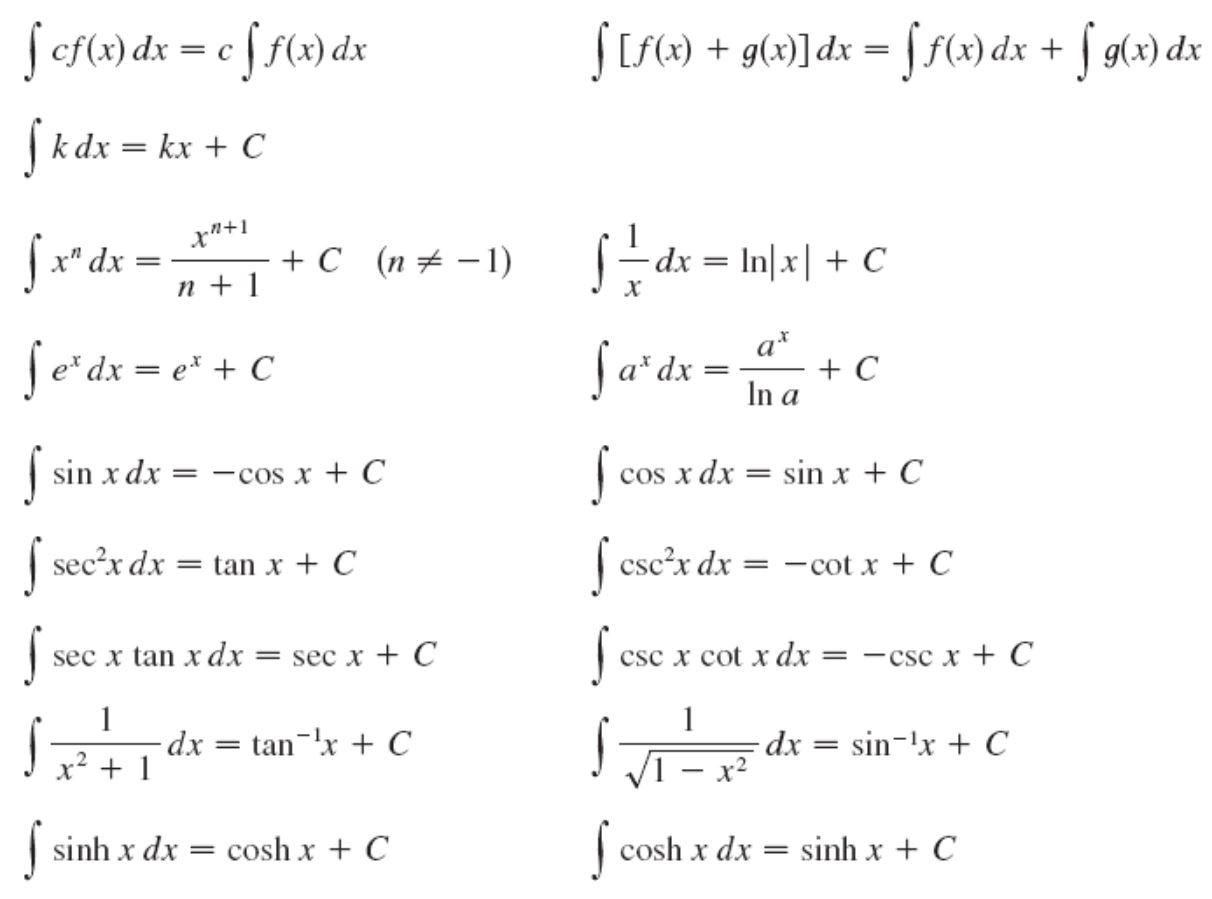
\includegraphics[width=0.85\textwidth]{media/indef-integrals.JPG}$$



\subsubsection{Net Change Theorem} The integral of a rate of change is the net change, $\int_a^b F'(x)dx = F(b)-F(a)$



\subsection{Day 22}

\subsubsection{Integration by Substitution}  A function $F$ is called an anti-derivative of $f$ on an interval $I$ if $F’(x)=f(x)$ for all $x$ in $I$.

\begin{enumerate}
    \item Let $u=g(x)$, where $g(x)$ is part of the integrand.
    \item Calculate $\frac{du}{dx}$ (or $g'(x)$)
    \item Use the substitution $u=g(x)$ and $du=g'(x)dx$ to convert the entire integral into one involving only $u$
    \item If indefinite, evaluate the resulting integral and plug in $u$ by $g(x)$.
    \item If definite, plug in the lower limit of the integral and the upper limit of the integral into the expression $u=g(x)$ and get the new lower and upper limits. Then, evaluate the new definite integral (involving only $u$) by finding the anti-derivative of $f$ and use the Fundamental Theorem.
\end{enumerate}

\subsubsection{Substitution Rule for Definite Integral}
If $g'$ is continuous on $[a,b]$ and $f$ is continuous on the range of $u=g(x)$, then

$$\int_a^b f(g(x)) \cdot g'(x) dx = \int_{g(a)}^{g(b)} f(u) du$$


\subsection{Day 23}

\subsubsection{One-to-One Function} A function $f$ that never takes one a same value twice; that is $f(x_1)\neq f(x_2)$ whenever $x_1\neq x_2$. 

$$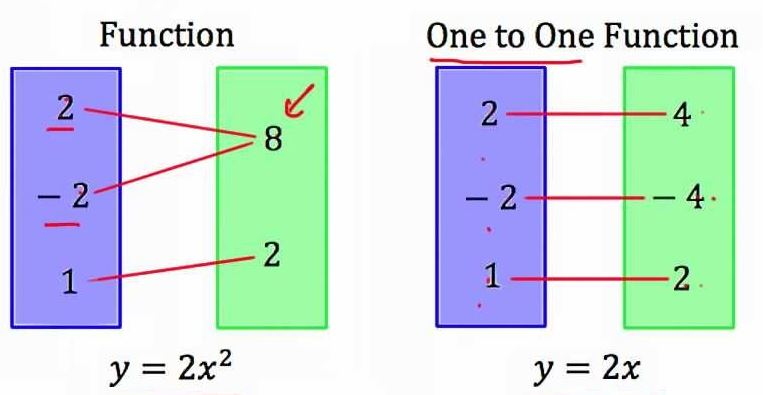
\includegraphics[width=0.65\textwidth]{media/onetoone.JPG}$$

\paragraph{Horizontal Line Test} If you draw a horizontal line through the graph, it should only intersect once if it's a 1-to-1 function.

\paragraph{Remark} All strictly increasing/decreasing functions are 1-to-1
\begin{itemize}
    \item $f'(a) > 0$ means strictly increasing
    \item $f'(a) < 0$ means strictly decreasing
\end{itemize}

\subsubsection{Inverse Function} Let function $f$ be a 1-to-1 function with domain $A$ and range $B$. Then its inverse function $f^{-1}$ has domain $B$ and range $A$ and is defined by $f^{-1}(y)=x \iff f(x)=y$ for any $y$ in $B$.

\paragraph{Remark} 
\begin{itemize}
    \item The domain of $f^{-1}$ is range of $f$
    \item The range of $f^{-1}$ is the domain of $f$
    \item $f^{-1}(f(x)) = x$
    \item $f(f^{-1}(x)) = x$
\end{itemize}


\paragraph{Steps to find inverse}
\begin{enumerate}
    \item Write $y=f(x)$
    \item Solve this equation for $x$ in terms of $y$
    \item To express $f^{-1}$ as a function of $x$, interchange $x$ and $y$.
\end{enumerate}

\subsubsection{Derivative of Inverse Function}\label{Derivative of Inverse Function}
If $f$ is a 1-to-1 differentiable function with inverse function $f^{-1}$, then the inverse function is differentiable and the following is true: 

$$(f^{-1})'(x) = \frac{1}{f'(f^{-1}(x))}$$




\section{Week 7}

\subsection{Day 25}

\subsubsection{Exponential Functions}
A function $f$ is  exponential if it is in the form $f(x)=a^x, a>0, a\neq 1$. 
\begin{itemize}
    \item If $a>1$, the range is $(0, \infty)$ and greater the $a$, greater the slope
    \item If $1>a>0$, the range is $(\infty, 0)$ and lower the $a$, greater the slope
\end{itemize}

\paragraph{Derivative of Exponential Function}
$$a^x \cdot \lim_{h\to0} \frac{a^h-1}{h} = a^x \cdot f'(0)$$

\subsubsection{$e$}
The function $f(x)=e^x$ is called the natural exponential function because the derivative is itself.

\subsection{Day 26}
\subsubsection{Log Functions:} Exponential functions are 1-to-1, hence it has an inverse function $f^{-1}$:

$$f^{-1} (x) = log_a x, x>0$$
$$y=log_a x \iff a^y = x$$

\noindent Therefore, if $a>1$ the function $f(x)=log_a x$ is a 1-to-1, continuous, increasing function with the domain $(0, \infty)$ and range $(-\infty, \infty)$. If $x$, $y>0$ and $r$ is any real number, then:

$$log_a(xy)=log_a x + log_a y$$
$$log_a(x/y)=log_a x - log_a y$$
$$log_a(x^r)=r\cdot log_a x$$

$$lim_{x\to \infty} [log_a x] = \infty$$
$$lim_{x\to 0^+} [log_a x] = -\infty, a > 1$$

\subsubsection{Inverse Function Rules:}

$$(f \circ f^{-1})(x) = a^{log_a x} = x, x>0$$
$$(f^{-1} \circ f)(x) = log_a (a^x) = x$$

\subsubsection{Theorem} If $f$ is a 1-to-1 differentiable function with the inverse function $f^{-1}$, then the inverse function is differentiable and we can use \ref{Derivative of Inverse Function}: 

$$(f^{-1})'(x) = \frac{1}{f'(f^{-1}(x))}$$

\subsection{Day 27}
$$\frac{d}{dx} \left( \sin^{-1} x \right) = \frac{1}{\sqrt{1-x^2}}, (-1 < x < 1) \text{ between } -\frac{\pi}{2} \leq y \leq \frac{\pi}{2}$$
$$\frac{d}{dx} \left( \cos^{-1} x \right) = -\frac{1}{\sqrt{1-x^2}}, (-1 < x < 1)  \text{ between } 0 \leq y \leq \pi$$
$$\frac{d}{dx} \left( \tan^{-1} x \right) = \frac{1}{1+x^2}, x \in {\mathbb{} R}\text{ between } -\frac{\pi}{2} \leq y \leq \frac{\pi}{2}$$

\subsection{Day 28}
\subsubsection{Indeterminate Forms:}

\begin{minipage}{0.45\textwidth}

$$ \frac{0}{0}$$
$$ \frac{\infty}{\infty}$$
$$ 0^0$$\hfill
\end{minipage}
\begin{minipage}{0.45\textwidth}

\begin{tabular}{|p{\textwidth}}

$$0 \cdot \infty (\neq{} 0)$$
$$\infty - \infty (\neq{} 0)$$
$$\infty^0$$

\end{tabular}
\end{minipage}

\subsubsection{L'Hospital's Rule:} Suppose $f$ and $g$ are differentiable and $g'(x) \neq{} 0$ on an open interval $I$ that contains $a$ (except possibly at $a$). Suppose that 

$$\lim_{x\to a} f(x)  = 0  \text{ and  } \lim_{x \to a} g(x) = 0$$
$$\text{or that } \lim_{x\to a} f(x)  = \pm \infty  \text{ and  } \lim_{x \to a} g(x) = \infty$$

\noindent (In other words, we have an indeterminate form of type $\frac{0}{0}$ or $\frac{\infty}{\infty}$.) Then

$$\lim_{x\to a} \frac{f(x)}{g(x)} = \lim_{x\to a} \frac{f'(x)}{g'(x)}$$

\noindent if the limit on the right side exists (or is $\infty$ or $-\infty$)



\section{Week 8}
\subsection{Day 29}
\subsubsection{Area Between Lines} The area $A$ of the region bounded by the curves $y=f(x),\ y = g(x),$ and the lines $x=a, x=b$, where $f$ and $g$ are continuous and $f(x)>g(x)$ for  all $x$ in $[a,b]$ is 
$$A = \int_a^b \left[ f(x) - g(x) \right] dx$$

\noindent Or, if we just want to find the area inclsed we can use 
$$A = \int_a^b \left| f(x) - g(x) \right| dx$$


\subsubsection{Average value of $f$}
We define the average value of $f$ on the interval $[a,b]$ as 
$$f_{avg}= \frac{1}{b-a} \cdot \int_a^b f(x) dx$$

\subsubsection{Mean Value Theorem for Integrals} If $f$ is continuous on $[a,b]$, then there exists a number $c$ in $[a,b]$ such that 

$$f(x) = f_{avg} = f(c) \cdot (b-a)$$


\subsection{Day 30}
\subsubsection{Area of Shape} Let $S$ be a solid that lies between $x=a$ and $x=b$. If the cross-sectional area of $S$ in the plane $P_x$, through $x$ and perpendicular to the $x$-axis, is $A(x)$, where $A$ is a continuous function, then the volume of $S$ is 

$$V=\lim_{n \to \infty} \sum_{i=1}^{n} A(x_i^*) \Delta x = \int_a^b A(x) dx$$

\subsubsection{Volume}

$$V=\int_a^b A(x) dx$$

\subsubsection{Disk}

$$A(x) = \pi \cdot r^2 \text{ if rotating about $x$-axis}$$

\subsubsection{Cross-Section (washer)}

$$A(x) = \pi \cdot (R^2 - r^2)  \text{ if rotating about $x$-axis}$$

\subsubsection{Cylinder}

$$A(x) = 2\pi x \cdot f(x) \cdot dx \text{ if rotating about $y$-axis}$$


\end{document}
